\documentclass{article}

\usepackage{listings} % For code formatting
\usepackage[utf8]{inputenc}  % For encoding support
\usepackage{amsmath}         % For mathematical formatting
\usepackage{graphicx}        % For including images
\usepackage{xcolor}
\usepackage[a4paper, left=0.5in, right=0.5in, top=0.5in, bottom=0.5in]{geometry}  % Adjust margins here
\usepackage{tcolorbox}
\usepackage{palatino}  % Use Inconsolata font (or replace with your choice)
\usepackage{amsmath, amssymb, array, booktabs}

% Define colors
\definecolor{codebg}{RGB}{240, 240, 240}  % Light gray background
\definecolor{framecolor}{RGB}{100, 100, 100}  % Dark gray frame
\definecolor{titlebg}{RGB}{30, 30, 30}  % Dark title background
\definecolor{titlefg}{RGB}{255, 255, 255}  % White title text

% Custom lstset
\lstset{
    language=C++,                    
    basicstyle=\ttfamily\footnotesize\fontfamily{zi4}\selectfont, % Use Inconsolata
    keywordstyle=\bfseries\color{blue},        
    commentstyle=\itshape\color{gray},        
    stringstyle=\color{red},          
    numbers=left,                     
    numberstyle=\tiny\color{blue},    
    frame=single,                     
    breaklines=true,                   
    captionpos=b,                      
    backgroundcolor=\color{codebg},  % Light gray background
    rulecolor=\color{framecolor},    % Dark frame
    tabsize=4                         
}

% Custom command to add a styled heading
\newtcbox{\codebox}{colback=titlebg, colframe=titlebg, colupper=titlefg, 
  boxrule=0pt, arc=5pt, left=5pt, right=5pt, top=3pt, bottom=3pt}

\title{Hybrid CPU/GPU Clustering in Shared Memory on the Billion Point Scale}

\author{Ayush Raina, 22148}
\date{\today}

\begin{document} 

\maketitle

\subsection*{Overview}
This paper introduces \textbf{BPS-HDbscan}, a high-performance clustering algorithm for billion-point datasets using a \textbf{shared-memory CPU/GPU} system. Built on DBSCAN, it avoids redundant distance calculations, efficiently partitions data to fit GPU memory, and leverages both CPU and GPU for parallel processing. Unlike previous methods that relied on distributed systems, BPS-HDbscan achieves scalability on a single machine, making it suitable for massive datasets in fields like astronomy.

\subsection*{Motivation}
Clustering is a core task in many scientific applications, particularly in astronomy, where data volumes are massive. For instance, the \textbf{Gaia mission} has produced a catalog of over \textbf{1.69 billion celestial objects}, and clustering such data is essential for understanding star formations and galactic structures. DBSCAN is a popular density-based clustering algorithm known for its ability to detect clusters of arbitrary shapes and handle noise. However, its inherent sequential design and high computational cost, especially for pairwise distance calculations, make it unsuitable for such large datasets without optimization. Existing parallel versions either rely on distributed-memory systems or are not memory-efficient. There is a clear need for a \textbf{shared-memory parallel approach} that can effectively utilize modern multi-core CPUs and many-core GPUs while staying within the memory limits of a single machine.

\subsection*{Methodology and Key Contributions}
BPS-HDbscan introduces several innovations to achieve high performance on large datasets. It reduces the number of expensive distance calculations by exploiting the density properties of the data and DBSCAN's input parameters. To address GPU memory limitations, it batches computations and partitions the dataset so that each partition fits into GPU memory. The algorithm executes these partitions in parallel, ensuring both the CPU and GPU remain fully utilized throughout the clustering process. It also incorporates efficient techniques for merging subclusters across partitions. These design choices, inspired by prior work, enable BPS-HDbscan to scale to a billion points on a single shared-memory machine—something that, until now, was only possible using large distributed systems.

\section{Leveraging Hybrid-Dbscan}

Hybrid-Dbscan computes the $\epsilon$-neighborhood of all points on the GPU, and the data is used by Dbscan for clustering on the CPU, thereby eliminating the need for CPU-based index searches. Compared to Hybrid-Dbscan, BPS-HDbscan supports datasets larger than GPU memory by partitioning the data, clustering partitions concurrently, and avoiding distance calculations in dense regions. Hybrid-Dbscan is limited to smaller datasets, while BPS-HDbscan is used for billion-point datasets.

\subsection{Indexing Scheme}
Hybrid-Dbscan uses a grid-based indexing scheme with cells of length $\epsilon$. For a given point, the $\epsilon$-neighborhood search checks the point's cell and its adjacent cells (9 total cells in 2D). We modify the indexing scheme to only index non-empty cells, reducing the size of the index and improving memory efficiency. The space complexity of the index is \(O(|D|)\), where \(|D|\) is the number of data points. In the worst case, the space complexity is \(4|D|\), allowing the GPU to process larger datasets or partitions.

\subsection{Batching Scheme}
Hybrid-Dbscan uses a batching scheme that allows the total result set size to exceed GPU memory capacity. The number of batches, \(n_b\), is determined by sampling the dataset and estimating the total result set size. This avoids the need for result set buffer overflow mitigation.

\[
\text{Total Size of Pinned Memory Buffers} = n_s \times b_s
\]

where \(n_s\) is the number of CUDA streams and \(b_s\) is the batch size. At a minimum, we set \(n_s = n_b = 3\) and \(b_s = 10^8\). When using two GPUs, the memory size is doubled.

\subsection{Overestimation Factor}
An overestimation factor \(\alpha = 0.25\) is used to account for reference points that have a larger search distance.

\[
\alpha = 0.25
\]

The key difference between \textbf{Hybrid-Dbscan} and the version used in this paper is that we \textbf{only index non-empty grid cells}. This change reduces memory usage since we store only the cells that contain data, as opposed to indexing all grid cells, including empty ones, which was the original approach.

\section{Dense Box Algorithm and Hybrid-Dbscan Clustering}

Section 4 describes the \textbf{DenseBox} algorithm combined with \textbf{Hybrid-Dbscan} clustering to improve computational efficiency by leveraging dense regions in the data. \\ \\
1. \textbf{Adjacency of Dense Boxes: }
Dense boxes are identified by partitioning the dataset into $\epsilon/(2\sqrt{2})$ cells. Adjacent dense boxes (containing points within $\epsilon$ distance) are merged, reducing the number of clusters. \\ \\ 
2. \textbf{Merging Non-Adjacent Dense Boxes: } 
Non-adjacent dense boxes are merged if points in separate boxes are within $\epsilon$ distance. This process further refines the clustering by connecting distant dense regions. \\ \\
3. \textbf{Merging Dense Boxes and Dbscan Clusters: }
\textbf{Hybrid-Dbscan} clusters are merged with dense boxes if points within the clusters are within $\epsilon$ of a point in a dense box. This ensures effective integration of Dbscan and DenseBox clusters. \\\\
4. \textbf{Detection of Dense Box Merges: }
Merges are detected using \textbf{reference points} placed in each non-empty cell. A 1.5$\epsilon$-neighborhood search around these reference points helps identify potential merges without costly neighborhood searches. \\ \\
5. \textbf{Merging Using Disjoint Sets: }
The \textbf{disjoint set data structure} efficiently handles cluster merges. It tracks merged clusters and updates final cluster assignments with a single scan, enabling scalability for large datasets. \\ \\ 
6. \textbf{Selectively Using the Dense Box Algorithm: } 
The DenseBox algorithm is selectively used based on the data distribution, $\epsilon$, and \texttt{minpts} values. A heuristic involving the average number of points per cell determines whether to use DenseBox or rely on Hybrid-Dbscan, ensuring computational efficiency.

\section{Clustering Large Datasets and BPS-HDbscan Algorithm}

When the dataset and algorithm components exceed the GPU's limited global memory, the dataset is divided into \(n_p\) partitions. Clustering occurs on each partition, followed by merging the results. Similarly, in distributed-memory implementations, partitioning ensures that each node can cluster separate dataset regions.

The dataset \(D\) is first sampled and binned along the first dimension. It is then partitioned into \(n_p\) subsets with roughly equal numbers of points. After clustering each partition, clusters are merged by detecting overlapping core points from neighboring partitions. Merging occurs when two clusters from neighboring partitions share a point in their \(\epsilon\)-neighborhood, with at least \(\texttt{minpts}\) neighbors.

Mathematically, the condition for merging two clusters is:
\[
\text{Core}(p_1, \texttt{minpts}) = \text{True} \quad \text{and} \quad \text{Core}(p_2, \texttt{minpts}) = \text{True},
\]
and if one point lies in the \(\epsilon\)-neighborhood of the other, the clusters containing \(p_1\) and \(p_2\) are merged.

The BPS-HDbscan algorithm uses this approach to partition and cluster the dataset. It takes as input the dataset \(D\), \(\epsilon\), \(\texttt{minpts}\), and the number of partitions \(n_p\). Initially, the cluster assignments for each partition are set to empty sets, and the dataset is partitioned. Each partition is processed independently, and DenseBox is optionally used to detect clusters. If DenseBox is enabled, it clusters points in the partition and returns a set of clusters \(C_{DBox}\) and a list of points \(L\) that could not be clustered. Reference points \(M\) are then generated, and a query set \(Q = L \cup M\) is formed. The neighbors of points in \(L\) and reference points in \(M\) are computed, and these neighbors are used as input for DBSCAN.

The final clusters for each partition are obtained by merging the results of DenseBox and DBSCAN. If DenseBox is not enabled, Hybrid-Dbscan is used instead. After all partitions are processed, the clusters are reconciled: clusters from neighboring partitions are merged, and noise points detected in individual partitions may form new clusters.

Parallelization is crucial for handling large datasets. The key steps, such as clustering, index construction, and neighbor table computation, are executed in parallel. GPU resources are specifically used for neighbor table computation, but only one thread per partition can access the GPU at a time to avoid conflicts.

The BPS-HDbscan algorithm efficiently handles large-scale datasets by partitioning the data, performing parallel clustering, and merging results across partitions, making it suitable for GPU-accelerated environments.

\begin{figure}[h]
    \centering
    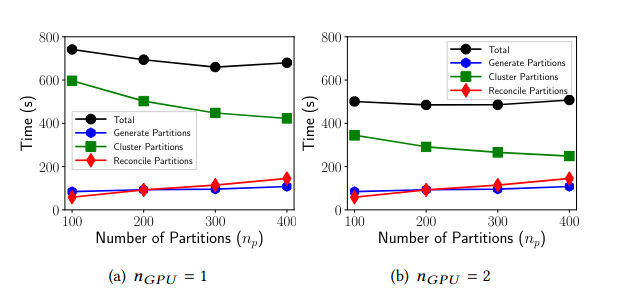
\includegraphics[width=0.4\textwidth]{result1.png}
    \caption{Response Time vs $n_p$ with \textbf{DBox-Off}, $\epsilon=0.01$, \texttt{minpts}=4,$n_c=4$}
    \label{fig:algorithm_overview}
\end{figure}
In the above $n_c$ denotes the number of partitions being concurrently clustered. There are various other results discussed in the paper, but we need to first discuss more concepts to understand the results and is difficult to summarize all in 3 pages.

\subsection*{Critical Analysis}
We have already discussed about key contributions in beginning of this report. The paper is well-structured and provides a clear overview of the problem. However there is further scope for improvements. The method is primarily tested on 2D spatial data, limiting its demonstrated applicability to low-dimensional domains. Its performance in high-dimensional clustering scenarios remains uncertain. Another aspect is that the DenseBox activation heuristic relies on a user-defined parameter $\mu$, which may require manual tuning and might not generalize well across all datasets. There's no direct, side-by-side performance comparison with the latest DBSCAN variants, which would help position its effectiveness more clearly. Most of other variants are not Hybrid Implementations.
\end{document}
